%%%%%%%%%%%%%%%%%%%%%%%%%%%%%%%%%%%%%
% Tracing Overhead
%%%%%%%%%%%%%%%%%%%%%%%%%%%%%%%%%%%%%


\subsection{Tracing overhead}
\label{subsec:lowtoh}
 - Table \ref{comet_sd_pMpAcg_BC_itn_p3.5}
 - Fig \ref{comet_chartAvg_sd_B_p3_5}, \ref{comet_chartAvg_sd_C_p3_5} 
 
\begin{table*}[]
\caption{Server: \textbf{comet} - 
 Stat: \textbf{sd} - 
 Tools: pinMain , pinAll , callgrind ,  
 Inputs: B , C ,  
 Nodes: 1 , 4 , 16 , 64 ,  
 Desc: Primary}
\label{comet_sd_pMpAcg_BC_itn_p3.5}\begin{center}
\begin{tabular}{|l|rrrrrrrr|r|}
\hline
                &   bt &   cg &    ep &    ft &   is &   lu &   mg &   sp &   GM \\
\hline
 pinMain.B.1    & 1.55 & 1.82 &  2.68 &  2.11 & 2.48 & 1.31 & 2.57 & 1.33 & 1.91 \\
 pinMain.B.4    & 1.76 & 1.85 &  1.92 &  1.74 & 1.79 & 1.77 & 1.83 & 1.76 & 1.80 \\
 pinMain.B.16   & 2.19 & 2.62 &  2.39 &  1.93 & 1.82 & 2.80 & 2.43 & 2.23 & 2.28 \\
 pinMain.B.64   & 2.45 & 2.72 &  2.45 &  1.99 & 4.34 & 4.56 & 2.31 & 2.46 & 2.79 \\
 \hline
 AVG            & 1.99 & 2.25 &  2.36 &  1.94 & 2.61 & 2.61 & 2.29 & 1.95 & \textbf{2.20} \\
 \hline
 pinAll.B.1     & 1.85 & 2.73 &  4.21 &  2.85 & 4.52 & 1.74 & 5.57 & 1.73 & 2.87 \\
 pinAll.B.4     & 2.63 & 3.11 &  3.41 &  2.86 & 3.03 & 2.82 & 3.10 & 2.76 & 2.96 \\
 pinAll.B.16    & 3.73 & 4.20 &  4.36 &  2.96 & 2.84 & 4.30 & 4.49 & 3.71 & 3.77 \\
 pinAll.B.64    & 4.22 & 4.19 &  4.55 &  3.13 & 5.46 & 4.73 & 4.17 & 4.23 & 4.29 \\
 \hline
 AVG            & 3.11 & 3.56 &  4.13 &  2.95 & 3.96 & 3.40 & 4.33 & 3.11 & \textbf{3.47} \\
 \hline
 callgrind.B.1  & 8.68 & 6.07 &  9.31 & 10.33 & 2.64 & 7.61 & 3.39 & 6.62 & 6.24 \\
 callgrind.B.4  & 6.13 & 3.63 &  2.95 &  3.50 & 1.46 & 5.41 & 1.43 & 5.98 & 3.34 \\
 callgrind.B.16 & 4.31 & 3.26 &  2.39 &  2.20 & 1.73 & 4.70 & 1.92 & 4.65 & 2.93 \\
 callgrind.B.64 & 2.85 & 2.71 &  1.86 &  2.16 & 4.13 & 4.10 & 1.87 & 3.54 & 2.77 \\
 \hline
 AVG            & 5.49 & 3.92 &  4.13 &  4.55 & 2.49 & 5.46 & 2.15 & 5.20 & \textbf{3.82} \\
 \hline
  \hline
 pinMain.C.1    & 1.41 & 1.29 &  2.51 &  1.90 & 2.34 & 1.12 & 1.76 & 1.11 & 1.61 \\
 pinMain.C.4    & 1.58 & 1.77 &  2.13 &  1.65 & 1.70 & 1.33 & 1.83 & 1.35 & 1.65 \\
 pinMain.C.16   & 1.82 & 2.39 &  2.47 &  1.52 & 1.83 & 2.22 & 2.40 & 1.82 & 2.03 \\
 pinMain.C.64   & 2.32 & 2.74 &  2.48 &  1.61 & 4.49 & 3.52 & 2.68 & 2.28 & 2.65 \\
 \hline
 AVG            & 1.78 & 2.05 &  2.40 &  1.67 & 2.59 & 2.05 & 2.17 & 1.64 & \textbf{1.98} \\
 \hline
 pinAll.C.1     & 1.47 & 1.55 &  3.25 &  2.00 & 3.06 & 1.26 & 2.52 & 1.20 & 1.90 \\
 pinAll.C.4     & 1.93 & 2.52 &  3.35 &  2.24 & 2.65 & 1.77 & 3.09 & 1.71 & 2.34 \\
 pinAll.C.16    & 2.70 & 3.47 &  4.27 &  2.15 & 2.80 & 3.21 & 4.30 & 2.75 & 3.13 \\
 pinAll.C.64    & 3.67 & 4.13 &  4.31 &  2.26 & 5.72 & 4.43 & 4.30 & 3.69 & 3.95 \\
 \hline
 AVG            & 2.44 & 2.92 &  3.79 &  2.16 & 3.56 & 2.67 & 3.55 & 2.34 & \textbf{2.83} \\
 \hline
 callgrind.C.1  & 8.52 & 4.51 & 13.47 & 13.13 & 3.81 & 7.93 & 6.31 & 5.15 & 7.13 \\
 callgrind.C.4  & 8.83 & 4.55 &  6.52 &  7.04 & 1.74 & 6.83 & 2.89 & 6.48 & 5.03 \\
 callgrind.C.16 & 6.87 & 4.00 &  3.55 &  2.87 & 1.87 & 6.61 & 2.31 & 6.56 & 3.89 \\
 callgrind.C.64 & 4.37 & 3.49 &  2.20 &  2.52 & 4.25 & 5.52 & 2.13 & 4.70 & 3.45 \\
 \hline
 AVG            & 7.15 & 4.14 &  6.44 &  6.39 & 2.92 & 6.72 & 3.41 & 5.72 & \textbf{4.88} \\
\hline
\end{tabular}
\end{center}
\end{table*}

   
Table \ref{comet_sd_pMpAcg_BC_itn_p3.5} shows the overhead caused by \parlotm, \parlota and  \callgrind on each application of NPB benchmark.
 Last column of table is showing the geometric mean of \textit{tracing overhead} by each tool for every application. \\
key strong points:
\begin{itemize}
\item On average, both \parlotm and \parlota has better performance than \callgrind and amount of informative data that \callgrind generates is smaller and less informative than other two
\item Why Callgrind scales better? [to be added]
\item Martin's question in the email [to be added]
\end{itemize}

\begin{figure}[!t]
\centering
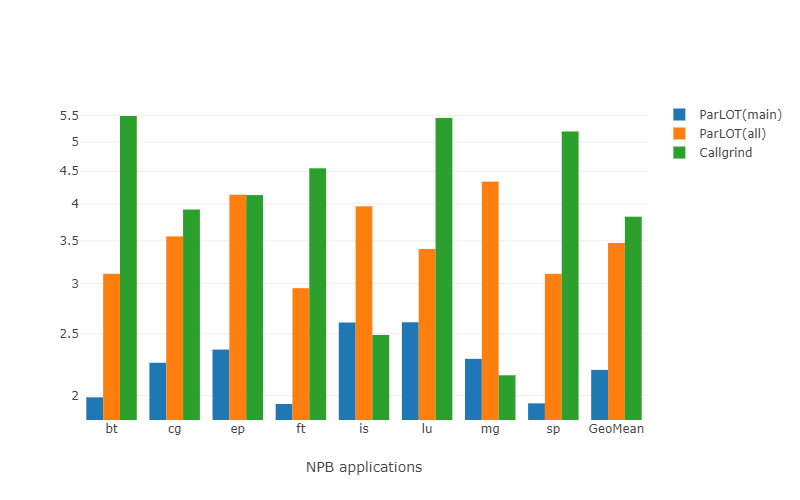
\includegraphics[width=3.9in]{figs.comet/comet_chartAvg_sd_B_p3_5.png}
\caption{ Input: \textbf{B} - Slowdown of \parlot(main,all) and \callgrind. Each bar is the average slowdown of each tool on each application for 1, 4 and 16 nodes (16, 64 and 256 cores). Last group of bars is GeoMean (from bold numbers in table \ref{comet_sd_pMpAcg_BC_itn_p3.5}). 
}
\label{comet_chartAvg_sd_B_p3_5}
\end{figure}


\begin{figure}[!t]
\centering
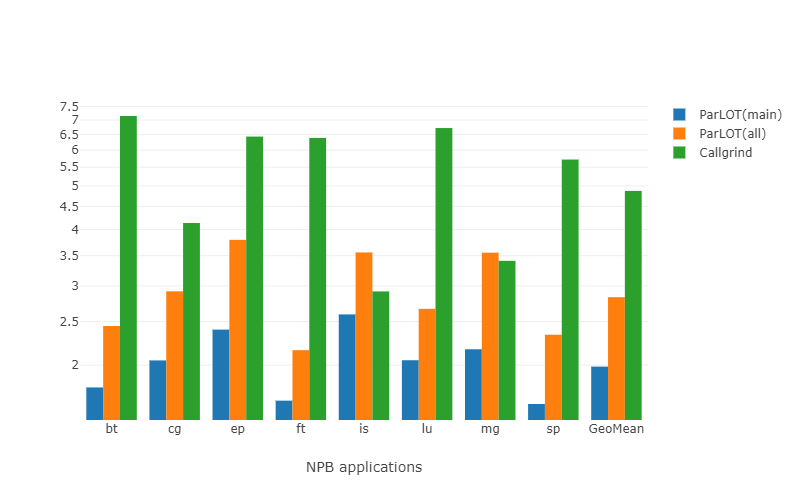
\includegraphics[width=3.9in]{figs.comet/comet_chartAvg_sd_C_p3_5.png}
\caption{ Input: \textbf{C} - Slowdown of \parlot(main,all) and \callgrind. Each bar is the average slowdown of each tool on each application for 1, 4 and 16 nodes (16, 64 and 256 cores). Last group of bars is GeoMean (from bold numbers in table \ref{comet_sd_pMpAcg_BC_itn_p3.5}). 
}
\label{comet_chartAvg_sd_C_p3_5}
\end{figure}



%%%%%%%%%%%%%%%%%%%%%%%%%%%%%%%%%%%%%
% Banwidth
%%%%%%%%%%%%%%%%%%%%%%%%%%%%%%%%%%%%%


  
\subsection{Required Bandwidth}
\label{subsec:lowbw}
 - Table \ref{comet_bw_pMpAcg_BC_itn_p3.5}
  - Fig \ref{comet_chartAvg_bw_B_p3_5}, \ref{comet_chartAvg_bw_C_p3_5}

Table \ref{comet_bw_pMpAcg_BC_itn_p3.5} shows the required bandwidth for each tool. 
In addition to big gap between average overhead of \parlotm and \callgrind, \parlotm also beats \callgrind in required bandwidth, especially for smaller inputs.
According to table \ref{comet_cr_pMpA_BC_itn_p3.5}, for example for \parlot(all) where the average compression ratio for input C is 644.38, and the correspondent required bandwidth which is 56.38, it shows that \parlot can collect almost 36 MB worth of data per core per second where it only needs 56.38 KB/S bandwidth.]


\begin{table*}[]
\caption{Server: \textbf{comet} - 
 Stat: \textbf{bw} - 
 Tools: pinMain , pinAll , callgrind ,  
 Inputs: B , C ,  
 Nodes: 1 , 4 , 16 , 64 ,  
 Desc: Primary
This table is showing the required bandwidth for each application (KiloBytes per core per second). $ReqBW_x = TraceSize_x (KB) / (\# of cores)_x / Runtime_x (S)$
. Clearly ParLOT(main) is beating Callgrind while they both generate the same information. ParLOT(all) bandwidth is the highest but with capturing all of the function calls within a single execution, there is no surprise. Figures \ref{comet_chartAvg_bw_B_p3_5} and \ref{comet_chartAvg_bw_C_p3_5} visualize these numbers (Average values) 
 }
\label{comet_bw_pMpAcg_BC_itn_p3.5}\begin{center}
\begin{tabular}{|l|rrrrrrrr|r|}
\hline
                &    bt &     cg &    ep &    ft &    is &     lu &    mg &     sp &    GM \\
\hline
 pinMain.B.1    &  4.72 &  21.86 &  3.83 &  1.52 &  0.79 &   2.39 &  5.62 &   5.36 &  3.69 \\
 pinMain.B.4    & 14.28 &  41.08 &  1.89 &  3.48 &  2.24 &  21.48 &  6.45 &  15.85 &  8.12 \\
 pinMain.B.16   & 14.31 &  46.59 &  1.45 &  4.86 &  3.40 &  31.79 &  6.53 &  18.55 &  9.41 \\
 pinMain.B.64   & 18.56 &  43.59 &  1.25 &  4.56 &  4.49 &  27.07 &  5.63 &  29.62 &  9.92 \\
 \hline
 AVG            & 12.97 &  38.28 &  2.10 &  3.60 &  2.73 &  20.68 &  6.06 &  17.35 &  \textbf{7.79} \\
 \hline
 pinAll.B.1     & 48.71 &  89.39 & 47.23 & 45.63 & 59.98 &  53.62 & 60.81 &  54.33 & 56.21 \\
 pinAll.B.4     & 61.84 & 101.23 & 45.21 & 55.12 & 53.20 &  71.09 & 54.85 &  73.62 & 62.68 \\
 pinAll.B.16    & 73.95 & 116.87 & 47.37 & 48.88 & 47.79 & 100.91 & 55.80 &  84.61 & 67.97 \\
 pinAll.B.64    & 81.80 & 110.15 & 44.16 & 47.98 & 37.84 & 100.26 & 52.67 &  99.90 & 66.47 \\
 \hline
 AVG            & 66.58 & 104.41 & 45.99 & 49.40 & 49.70 &  81.47 & 56.03 &  78.12 & \textbf{63.33} \\
 \hline
 callgrind.B.1  &  1.57 &   7.69 &  7.39 &  4.56 & 39.49 &   2.61 & 34.41 &   2.71 &  6.67 \\
 callgrind.B.4  &  6.51 &  16.01 & 22.10 & 15.65 & 45.46 &   8.63 & 45.47 &   7.78 & 16.31 \\
 callgrind.B.16 & 17.20 &  24.62 & 37.42 & 23.84 & 29.87 &  16.23 & 51.49 &  15.81 & 24.93 \\
 callgrind.B.64 & 26.82 &  27.65 & 45.93 & 25.14 & 11.04 &  17.75 & 45.27 &  20.20 & 25.02 \\
 \hline
 AVG            & 13.03 &  18.99 & 28.21 & 17.30 & 31.47 &  11.30 & 44.16 &  11.62 & \textbf{18.23} \\
 \hline
 \hline
 pinMain.C.1    &  1.82 &  16.96 &  5.15 &  1.16 &  0.69 &   0.77 &  3.56 &   1.40 &  2.17 \\
 pinMain.C.4    &  7.53 &  44.87 &  3.00 &  2.50 &  2.12 &  20.13 &  7.08 &  13.74 &  7.55 \\
 pinMain.C.16   & 16.30 &  55.04 &  1.84 &  6.10 &  3.35 &  34.09 &  7.24 &  20.68 & 10.70 \\
 pinMain.C.64   & 17.45 &  61.43 &  1.30 &  5.93 &  4.42 &  38.28 &  5.62 &  26.09 & 10.94 \\
 \hline
 AVG            & 10.77 &  44.58 &  2.82 &  3.92 &  2.65 &  23.32 &  5.88 &  15.48 &  \textbf{7.84} \\
 \hline
 pinAll.C.1     & 17.80 &  53.37 & 26.34 & 20.89 & 48.31 &  25.31 & 52.61 &  19.46 & 29.99 \\
 pinAll.C.4     & 51.78 &  95.84 & 36.80 & 43.82 & 51.40 &  58.39 & 54.18 &  65.77 & 55.15 \\
 pinAll.C.16    & 75.38 & 121.03 & 44.29 & 61.39 & 46.90 & 101.05 & 56.49 & 101.32 & 71.37 \\
 pinAll.C.64    & 80.63 & 135.19 & 43.49 & 46.28 & 37.09 & 117.87 & 54.05 &  99.02 & 68.99 \\
 \hline
 AVG            & 56.40 & 101.36 & 37.73 & 43.09 & 45.93 &  75.66 & 54.33 &  71.39 & \textbf{56.38} \\
 \hline
 callgrind.C.1  &  0.40 &   3.09 &  1.96 &  1.05 & 14.60 &   0.70 &  6.96 &   0.75 &  1.85 \\
 callgrind.C.4  &  1.78 &   8.87 &  7.74 &  4.48 & 31.74 &   2.82 & 21.03 &   2.78 &  6.41 \\
 callgrind.C.16 &  6.01 &  15.82 & 22.86 & 10.75 & 26.50 &   7.45 & 39.05 &   6.96 & 13.72 \\
 callgrind.C.64 & 14.32 &  19.56 & 35.75 & 12.17 & 11.07 &  11.86 & 40.69 &  12.83 & 17.39 \\
 \hline
 AVG            &  5.63 &  11.84 & 17.08 &  7.11 & 20.98 &   5.71 & 26.93 &   5.83 &  \textbf{9.84} \\
\hline
\end{tabular}
\end{center}
\end{table*}



\begin{figure}[!t]
\centering
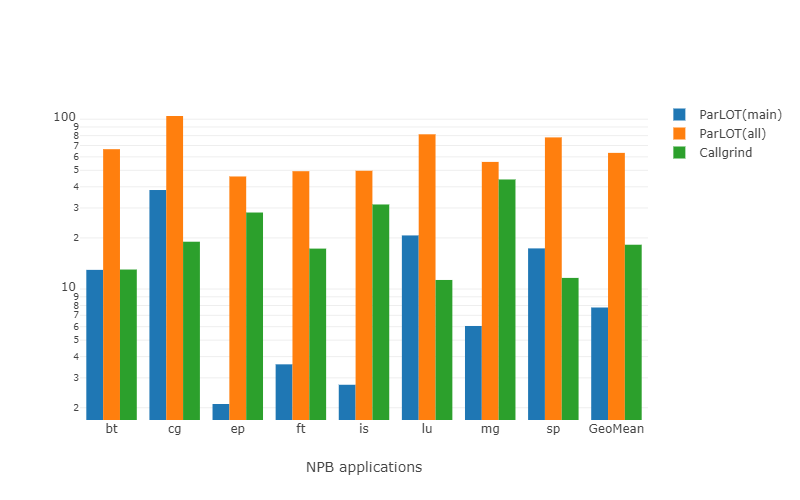
\includegraphics[width=3.5in]{figs.comet/comet_chartAvg_bw_B_p3_5.png}
\caption{ Input: \textbf{B} - Required Bandwidth per core (kB/s)
}
\label{comet_chartAvg_bw_B_p3_5}
\end{figure}



\begin{figure}[!t]
\centering
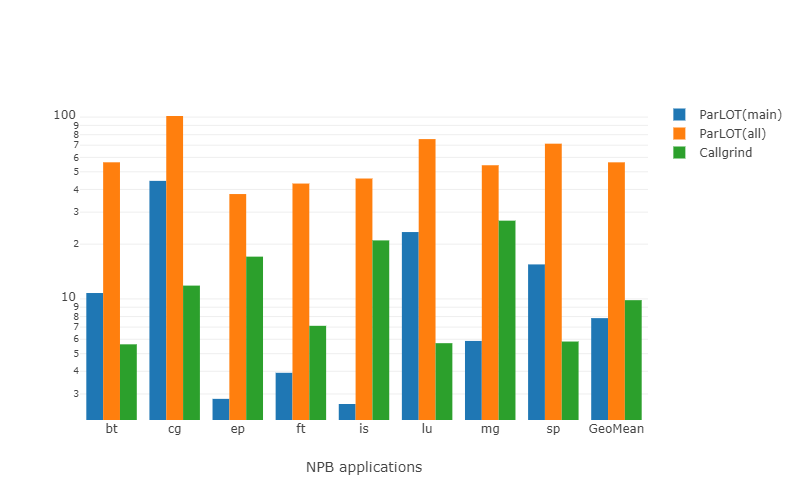
\includegraphics[width=3.5in]{figs.comet/comet_chartAvg_bw_C_p3_5.png}
\caption{ Input: \textbf{C}  - Required Bandwidth per core (kB/s)
}
\label{comet_chartAvg_bw_C_p3_5}
\end{figure}


%%%%%%%%%%%%%%%%%%%%%%%%%%%%%%%%%%%%%%%%%%%%%%%%%%%%%%%%%%%%%%%%%%%%%%%%%%%%%%%%%%
  
\subsection{Compression Ratio}
\label{subsec:cr}
 - Table \ref{comet_cr_pMpA_BC_itn_p3.5}
  - Fig \ref{comet_chartAvg_cr_B_p3_5}, \ref{comet_chartAvg_cr_C_p3_5}

  Table \ref{comet_cr_pMpA_BC_itn_p3.5} shows the compression ratios for all configs and inputs. On average, \parlot can store up to more than 1700 MB of collected data in just 1 MB trace files. Compression ratios are higher for larger input sizes (WHY?). Also \parlotm has better performance than \parlota (WHY?).
  

\begin{table*}[]
\caption{Server: \textbf{comet} - 
 Stat: \textbf{cr} - 
 Tools: pinMain , pinAll ,  
 Inputs: B , C ,  
 Nodes: 1 , 4 , 16 , 64 ,  
 Desc: Primary}
\label{comet_cr_pMpA_BC_itn_p3.5}\begin{center}
\begin{tabular}{|l|rrrrrrrr|r|}
\hline
              &      bt &     cg &       ep &       ft &       is &     lu &     mg &      sp &      GM \\
\hline
 pinMain.B.1  & 3035.93 &  94.35 & 12456.18 & 12173.49 &  9718.38 & 167.72 &  99.08 &  878.27 & 1255.17 \\
 pinMain.B.4  &  586.64 &  82.48 & 10368.41 &  1737.09 &   909.20 & 140.29 & 254.95 &  338.16 &  559.36 \\
 pinMain.B.16 &  346.66 & 113.28 &  8563.85 &  1077.35 &  1200.57 & 178.98 & 387.63 &  123.02 &  496.83 \\
 pinMain.B.64 &  252.24 & 147.78 &  7611.04 &  1122.62 &  1907.95 & 366.80 & 437.31 &  152.91 &  591.11 \\
 \hline
 AVG          & 1055.37 & 109.47 &  9749.87 &  4027.64 &  3434.03 & 213.45 & 294.74 &  373.09 &  \textbf{725.62} \\
 \hline
 pinAll.B.1   &  514.51 & 137.41 &  3335.77 &  1226.74 &   543.18 & 314.63 & 260.87 &  303.88 &  500.21 \\
 pinAll.B.4   &  315.71 & 137.21 &  1266.92 &   436.15 &   316.16 & 287.25 & 329.57 &  199.66 &  330.70 \\
 pinAll.B.16  &  226.86 & 181.58 &  1246.66 &  1026.53 &   927.09 & 299.30 & 469.29 &  171.52 &  430.39 \\
 pinAll.B.64  &  329.23 & 247.30 &  1394.07 &  1043.94 &  1984.62 & 410.32 & 548.47 &  307.16 &  597.55 \\
 \hline
 AVG          &  346.58 & 175.88 &  1810.86 &   933.34 &   942.76 & 327.88 & 402.05 &  245.56 &  \textbf{464.71} \\
 \hline
 \hline
 pinMain.C.1  & 8618.95 & 111.16 & 13067.96 & 21335.57 & 21856.49 & 350.03 & 247.44 & 1977.43 & 2371.35 \\
 pinMain.C.4  & 1910.64 & 110.45 & 12418.66 &  6520.34 &  2256.56 & 112.77 & 267.98 &  472.68 &  928.16 \\
 pinMain.C.16 &  580.79 & 133.24 & 11017.36 &  1239.31 &  1347.88 & 164.47 & 396.86 &  143.13 &  582.78 \\
 pinMain.C.64 &  322.83 & 131.92 &  9154.99 &  1065.12 &  1896.25 & 223.69 & 465.74 &  168.89 &  585.74 \\
 \hline
 AVG          & 2858.30 & 121.69 & 11414.74 &  7540.09 &  6839.30 & 212.74 & 344.50 &  690.53 & \textbf{1117.01} \\
 \hline
 pinAll.C.1   & 2579.37 & 181.76 &  7376.96 &  5143.08 &  1520.42 & 408.21 & 314.77 &  650.73 & 1107.37 \\
 pinAll.C.4   &  448.61 & 161.32 &  3194.58 &  1062.94 &   527.34 & 274.70 & 319.35 &  237.43 &  477.42 \\
 pinAll.C.16  &  285.05 & 185.74 &  1765.49 &   588.86 &  1106.34 & 273.63 & 467.35 &  141.69 &  426.92 \\
 pinAll.C.64  &  290.00 & 214.68 &  1512.89 &  1237.30 &  2038.72 & 329.04 & 496.21 &  270.83 &  565.82 \\
 \hline
 AVG          &  900.76 & 185.88 &  3462.48 &  2008.05 &  1298.21 & 321.39 & 399.42 &  325.17 &  \textbf{644.38} \\
\hline
\end{tabular}
\end{center}
\end{table*}



\begin{figure}[!t]
\centering
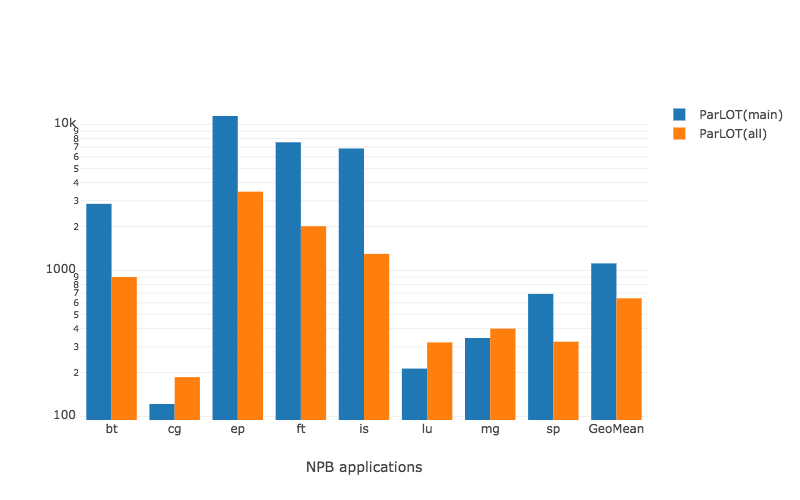
\includegraphics[width=3.5in]{figs.comet/comet_chartAvg_cr_C_p3_5.png}
\caption{ Input: \textbf{C}  - Compression Ratio
}
\label{comet_chartAvg_cr_C_p3_5}
\end{figure}


\begin{figure}[!t]
\centering
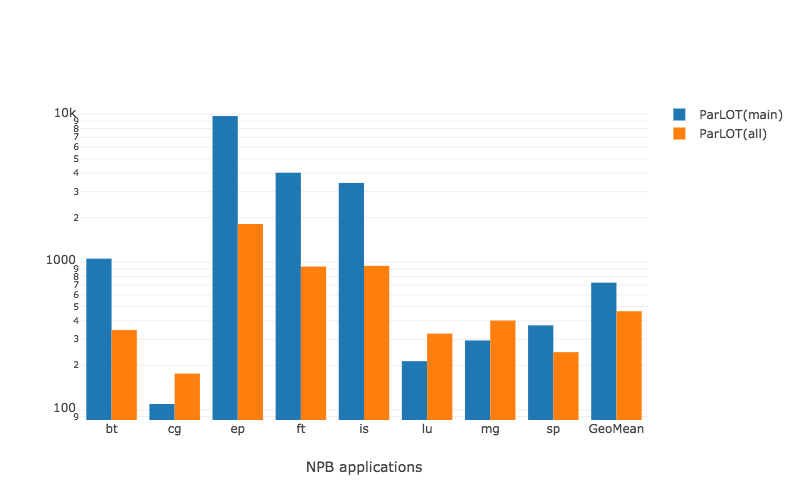
\includegraphics[width=3.5in]{figs.comet/comet_chartAvg_cr_B_p3_5.png}
\caption{ Input: \textbf{B}  - Compression Ratio
}
\label{comet_chartAvg_cr_B_p3_5}
\end{figure}
  
%%%%%%%%%%%%%%%%%%%%%%%%%%%%%%%%%%%%%%%%%%%%%%%%%%%%%%%%%%%%%  
  
\subsection{Pin-init Overhead} 
\label{subsec:pinit}
 - Table \ref{comet_wo_det_All_all_B_p3.5}, \ref{comet_wo_det_Main_all_B_p3.5}
  - Fig \ref{comet_chartDet_B_wc_byTool_p3_5}, \ref{comet_chartDet_C_wc_byTool_p3_5}
   Tables \ref{comet_wo_det_Main_all_B_p3.5}, \ref{comet_wo_det_All_all_B_p3.5} show average overhead added to each application by different variations of \parlot. Last row of tables shows geometric mean of each of its above values showing how much each phase of \parlot slows down the native execution. In general, we all expect that the added overhead of  Pin-init < \parlot < \parlotnc. Highlighted cells in tables are the ones which do not follow the above order. Number of highlighted cells for \parlot(main) is larger than \parlot(all). Variability of runtimes for \parlot(main) is more than other ones (native run, \parlot(all) and \callgrind) [new error bars to be added].
	
	
\begin{table*}[]
\caption{Server: \textbf{comet} - 
 Stat: \textbf{sd} - 
 Tools:  
 Inputs: B ,  
 Nodes: 1 , 4 , 16 , 64 ,  
 Desc: Detail Report}
\begin{center}
\label{comet_wo_det_Main_all_B_p3.5}
\scalebox{0.95}{
\begin{tabular}{|c|c|rrr|rrr|rrr|rrr|} 
\hline 
\multicolumn{1}{|l|}{\multirow{2}{*}{\textbf{Input: B}}} & \multicolumn{1}{r|}{Nodes :}    & \multicolumn{3}{c|}{1}  & \multicolumn{3}{c|}{4} & \multicolumn{3}{c|}{16}  & \multicolumn{3}{c|}{64} \\ \cline{2-14} 
\multicolumn{1}{|l|}{} & \multicolumn{1}{r|}{Detail Tools:} & \multicolumn{1}{c}{npin} & \multicolumn{1}{c}{ParLOT} & \multicolumn{1}{c|}{wpin} & \multicolumn{1}{c}{npin} & \multicolumn{1}{c}{ParLOT} & \multicolumn{1}{c|}{wpin} & \multicolumn{1}{c}{npin} & \multicolumn{1}{c}{ParLOT} & \multicolumn{1}{c|}{wpin} & \multicolumn{1}{c}{npin} & \multicolumn{1}{c}{ParLOT} & \multicolumn{1}{c|}{wpin} \\
\hline
\multirow{9}{*}{Main} &  bt  &  1.50  &  1.55  &   5.66  &  1.74  &  1.76  &  5.19  &  2.21  & \cellcolor{blue!25} 2.19  &  5.98  &  2.29  &  2.45  &  5.42 \\
 &  cg  &  1.75  &  1.82  &   2.39  &  1.95  & \cellcolor{blue!25} 1.85  &  2.64  &  2.72  & \cellcolor{blue!25} 2.62  &  5.06  &  2.67  &  2.72  &  7.01 \\
 &  ep  &  2.97  & \cellcolor{blue!25} 2.68  &  21.44  &  2.07  & \cellcolor{blue!25} 1.92  &  5.82  &  2.58  & \cellcolor{blue!25} 2.39  &  3.76  &  2.81  & \cellcolor{blue!25} 2.45  &  2.85 \\
 &  ft  &  1.87  &  2.11  &   6.29  &  1.76  & \cellcolor{blue!25} 1.74  &  2.85  &  2.13  & \cellcolor{blue!25} 1.93  &  2.25  &  2.23  & \cellcolor{blue!25} 1.99  &  2.22 \\
 &  is  &  2.51  & \cellcolor{blue!25} 2.48  &   4.87  &  1.80  & \cellcolor{blue!25} 1.79  &  2.08  &  2.11  & \cellcolor{blue!25} 1.82  &  1.90  &  4.76  & \cellcolor{blue!25} 4.34  &  5.75 \\
 &  lu  &  1.32  & \cellcolor{blue!25} 1.31  &   1.44  &  1.77  &  1.77  &  2.27  &  2.74  &  2.80  &  3.63  &  3.05  &  4.56  &  6.64 \\
 &  mg  &  2.64  & \cellcolor{blue!25} 2.57  &   2.80  &  1.75  &  1.83  &  1.79  &  2.64  & \cellcolor{blue!25} 2.43  &  2.73  &  2.37  & \cellcolor{blue!25} 2.31  &  2.49 \\
 &  sp  &  1.35  & \cellcolor{blue!25} 1.33  &   2.47  &  1.74  &  1.76  &  3.72  &  2.15  &  2.23  &  2.52  &  2.29  &  2.46  &  3.65 \\
 &  GM  &  1.90  &  1.91  &   4.15  &  1.82  & \cellcolor{blue!25} 1.80  &  3.03  &  2.40  & \cellcolor{blue!25} 2.28  &  3.24  &  2.72  &  2.79  &  4.12 \\
\hline 
\end{tabular} }

\end{center}
\end{table*}


\begin{table*}[]
\caption{Server: \textbf{comet} - 
 Stat: \textbf{sd} - 
 Tools:  
 Inputs: B ,  
 Nodes: 1 , 4 , 16 , 64 ,  
 Desc: Detail Report}
\begin{center}
\label{comet_wo_det_All_all_B_p3.5}
\scalebox{0.95}{
\begin{tabular}{|c|c|rrr|rrr|rrr|rrr|} 
\hline 
\multicolumn{1}{|l|}{\multirow{2}{*}{\textbf{Input: B}}} & \multicolumn{1}{r|}{Nodes :}    & \multicolumn{3}{c|}{1}  & \multicolumn{3}{c|}{4} & \multicolumn{3}{c|}{16}  & \multicolumn{3}{c|}{64} \\ \cline{2-14} 
\multicolumn{1}{|l|}{} & \multicolumn{1}{r|}{Detail Tools:} & \multicolumn{1}{c}{npin} & \multicolumn{1}{c}{ParLOT} & \multicolumn{1}{c|}{wpin} & \multicolumn{1}{c}{npin} & \multicolumn{1}{c}{ParLOT} & \multicolumn{1}{c|}{wpin} & \multicolumn{1}{c}{npin} & \multicolumn{1}{c}{ParLOT} & \multicolumn{1}{c|}{wpin} & \multicolumn{1}{c}{npin} & \multicolumn{1}{c}{ParLOT} & \multicolumn{1}{c|}{wpin} \\
\hline
\multirow{9}{*}{All} &  bt  &  1.76  &  1.85  &   6.23  &  2.39  &  2.63  &  6.39  &  3.40  &  3.73  &  10.64  &  3.74  &  4.22  &   9.47 \\
 &  cg  &  2.72  &  2.73  &   3.80  &  2.88  &  3.11  &  4.64  &  4.08  &  4.20  &  16.45  &  4.10  &  4.19  &  14.32 \\
 &  ep  &  4.42  & \cellcolor{blue!25} 4.21  &  23.24  &  3.25  &  3.41  &  7.16  &  4.27  &  4.36  &   5.67  &  4.43  &  4.55  &   5.13 \\
 &  ft  &  2.82  &  2.85  &   6.98  &  2.65  &  2.86  &  3.85  &  2.96  &  2.96  &   4.66  &  3.60  & \cellcolor{blue!25} 3.13  &   3.91 \\
 &  is  &  4.67  & \cellcolor{blue!25} 4.52  &   7.14  &  2.89  &  3.03  &  3.45  &  3.02  & \cellcolor{blue!25} 2.84  &   3.46  &  5.43  &  5.46  &  11.41 \\
 &  lu  &  1.71  &  1.74  &   2.41  &  2.54  &  2.82  &  4.91  &  4.09  &  4.30  &  11.60  &  4.48  &  4.73  &  25.53 \\
 &  mg  &  4.93  &  5.57  &   5.66  &  2.80  &  3.10  &  3.17  &  4.35  &  4.49  &   5.34  &  3.98  &  4.17  &   5.31 \\
 &  sp  &  1.70  &  1.73  &   3.13  &  2.54  &  2.76  &  5.32  &  3.43  &  3.71  &   7.39  &  3.66  &  4.23  &  22.13 \\
 &  GM  &  2.82  &  2.87  &   5.74  &  2.73  &  2.96  &  4.69  &  3.66  &  3.77  &   7.21  &  4.14  &  4.29  &   9.91 \\
\hline 
\end{tabular} }

\end{center}
\end{table*}


\begin{figure}[!t]
\centering
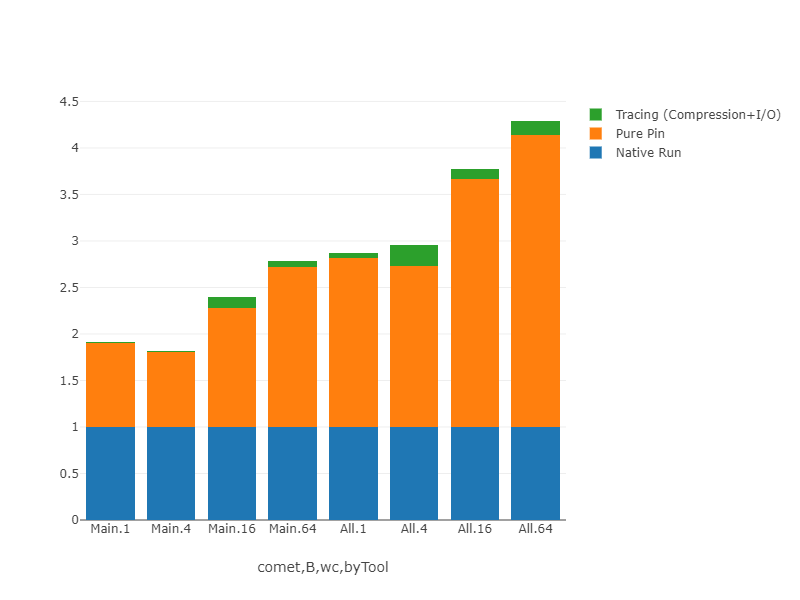
\includegraphics[width=4in]{figs.comet/comet_chartDet_B_wc_byTool_p3_5.png}
\caption{ Input: \textbf{B} - This figure and figure \ref{comet_chartDet_C_wc_byTool_p3_5} shows how much of the overhead of \parlot is caused by \pin and its initialization and how much by that section of \parlot that collects traces and compress them. It seems that overhead added by pure \pin does not scale well and increases with growing number of cores.
}
\label{comet_chartDet_B_wc_byTool_p3_5}
\end{figure}


\begin{figure}[!t]
\centering
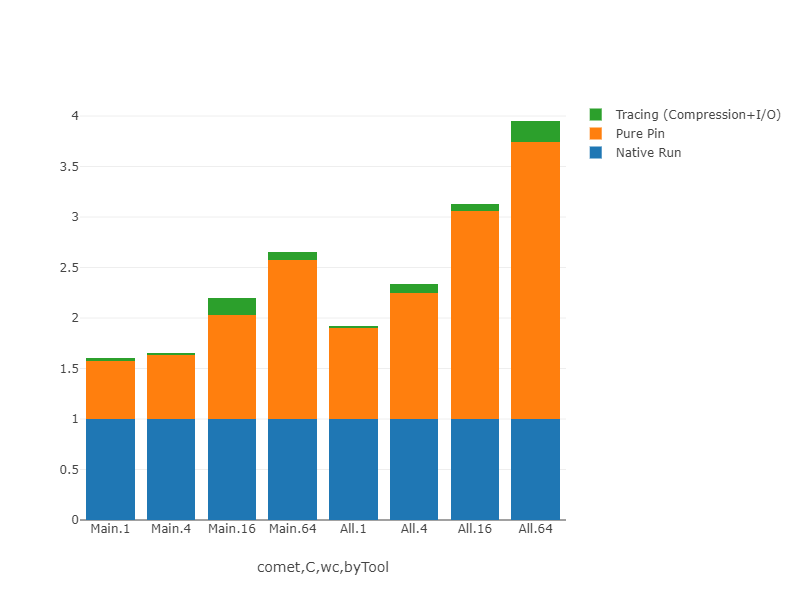
\includegraphics[width=4in]{figs.comet/comet_chartDet_C_wc_byTool_p3_5.png}
\caption{ Input: \textbf{C}
}
\label{comet_chartDet_C_wc_byTool_p3_5}
\end{figure}











\subsection{Compression impact} 
\label{subsec:compact}
\parlot without compression is terrible. (high impact of compression method on performance)
 - Table \ref{comet_wo_det_All_all_B_p3.5}, \ref{comet_wo_det_Main_all_B_p3.5}
   - Fig \ref{comet_chartDet_B_woc_byTool_p3_5}, \ref{comet_chartDet_C_woc_byTool_p3_5}
   
Figures \ref{comet_chartDet_B_wc_byTool_p3_5}, \ref{comet_chartDet_C_wc_byTool_p3_5}, \ref{comet_chartDet_B_woc_byTool_p3_5} and \ref{comet_chartDet_C_woc_byTool_p3_5} clearly show the performance of \parlot and impact of \parlot 's compression mechanism.
	


\begin{figure}[!t]
\centering
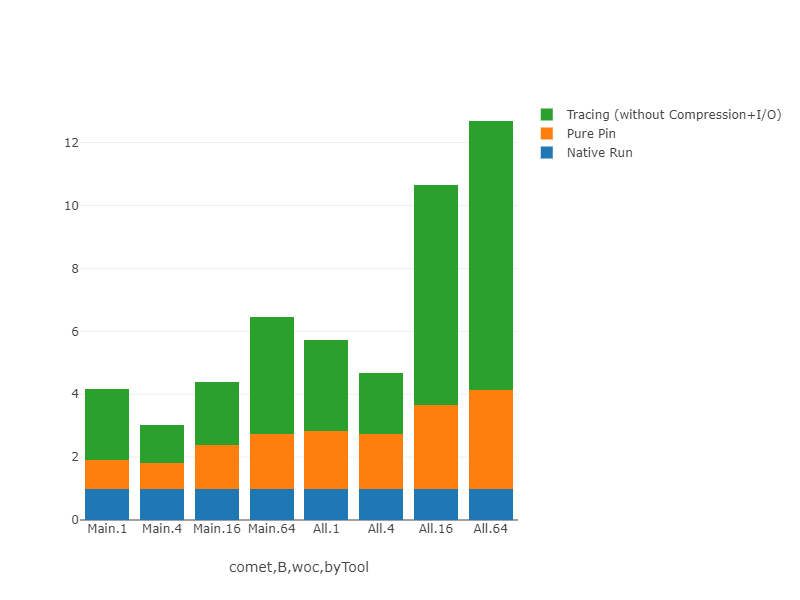
\includegraphics[width=4in]{figs.comet/comet_chartDet_B_woc_byTool_p3_5.png}
\caption{ Input: \textbf{B}- This figure and figure \ref{comet_chartDet_C_woc_byTool_p3_5} shows the impact of \parlot 's data compression.
}
\label{comet_chartDet_B_woc_byTool_p3_5}
\end{figure}

\begin{figure}[!t]
\centering
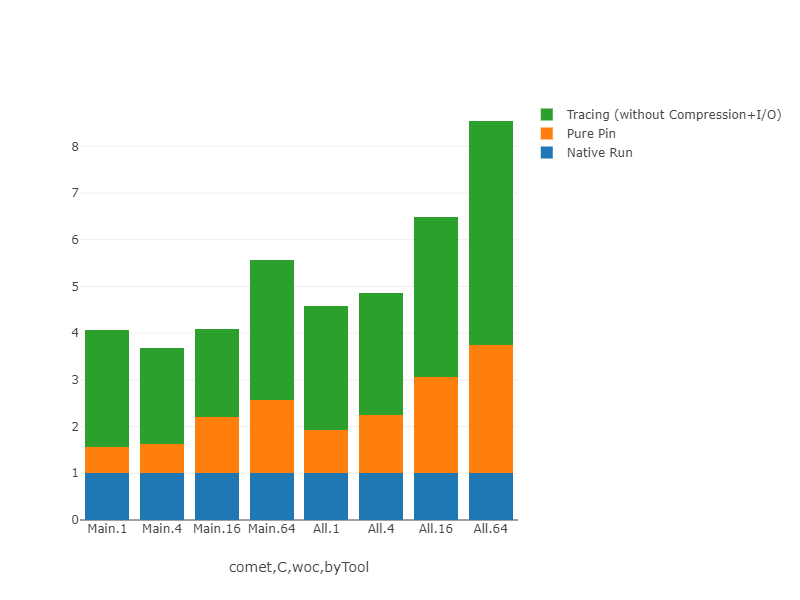
\includegraphics[width=4in]{figs.comet/comet_chartDet_C_woc_byTool_p3_5.png}
\caption{ Input: \textbf{C}
}
\label{comet_chartDet_C_woc_byTool_p3_5}
\end{figure}



